\documentclass[../main.tex]{subfiles}

\graphicspath{{../images/}}

\begin{document}
\pagestyle{fancy}
\lhead{Homework 10}
\chead{Junseo Shin}
\rhead{PHYS 421}

%  HW 6: 6.3, 6.5, 6.9, 6.10, 6.25
\begin{center}
    \section*{Homework 10}
    % add to toc
    \addcontentsline{toc}{section}{Homework 10}
\end{center}

\paragraph{6.3} Force of attractive between two magnetic dipoles $\vb m_1, \vb m_2$ a distance $r$ apart:
\begin{itemize}
    \item [(a)]  Given
    \begin{align*} \tag{6.2}    
        F = 2\pi I R B \cos\theta
    \end{align*}
    and
    \begin{align*}
        m_2 = I A = \pi I R^2
    \end{align*}
    The magnetic field due to $m_1$ is
    \begin{align*} \tag{5.89} \label{eq:hw10_89}
        \vb B_\text{dip} = \frac{\mu_0}{4\pi} \frac{1}{r^3} \qt[
            3 (\vb m \vdot \vu r) \vu r - \vb m
        ]
    \end{align*}
    
    \begin{figure*}[ht]
        \centering
        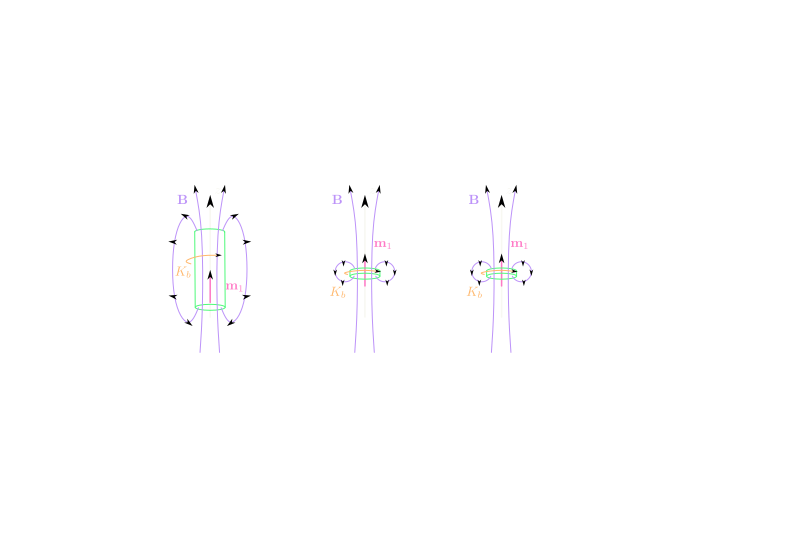
\includegraphics[width=0.6\textwidth]{hw10_1.png}
        \caption{Magnetic field due to a magnetic dipole $\vb m_1$}
        \label{fig:hw10_1}
    \end{figure*}
    \begin{align*}
        B \cos\theta &= \vb B_1 \vdot \vu y \\
        &= \frac{\mu_0}{4\pi} \frac{1}{r^3} \qt[
            3 (\vb m_1 \vdot \vu r) (\vu r \vdot \vu y) - \vb m_1 \vdot \vu y
        ] 
    \end{align*}
    and from Fig. \ref{fig:hw10_1}
    \begin{align*}
        \vb m_1 \vdot \vu r &= m_1 \cos\phi, \quad \vu r \vdot \vu y = \sin\phi,
        \quad \vu m_1 \vdot \vu y = 0 \\
        \qand \sin\phi & = \frac{R}{r}, \quad \cos\phi = \frac{z}{r} = \frac{\sqrt{r^2 - R^2}}{r}
    \end{align*}
    we get
    \begin{align*}
        B \cos\theta &= \frac{\mu_0}{4\pi} \frac{1}{r^3} \qt[
            3 m_1 \cos\phi \sin\phi - 0
        ] \\
        &= \frac{3 \mu_0}{4\pi} \frac{m_1}{r^3} \sin\phi \cos\phi \\
        &= \frac{3 \mu_0}{4\pi} m_1 R \frac{\sqrt{r^2 - R^2}}{r^5} \\
    \end{align*}
    So
    \begin{align*}
        F &= 2\pi I R B \cos\theta \\
        &= 2 (\pi I R^2) \frac{3 \mu_0}{4\pi} m_1 \frac{\sqrt{r^2 - R^2}}{r^5}
        &= \frac{3 \mu_0}{2\pi} m_1 m_2 \frac{\sqrt{r^2 - R^2}}{r^5}
    \end{align*}    
    where $r \gg R$ for the dipole so
    \begin{align*}
        \frac{\sqrt{r^2 - R^2}}{r^5} \approx \frac{\sqrt{r^2}}{r^5} = \frac{1}{r^4}
    \end{align*}
    Therefore
    \begin{align*}
        \boxed{F = \frac{3 \mu_0}{2\pi} \frac{m_1 m_2}{r^4}}
    \end{align*}
    \item [(b)] Using
    \begin{align*} \tag{6.3} \label{eq:hw10_3}
        \vb F = \grad(\vb m \vdot \vb B)
    \end{align*}
    and product rule (ii)
    \begin{align*}
        \vb F &= \grad(\vb m_2 \vdot \vb B) \\
        &= \vb m_2 \cross (\curl \vb B) + \vb B \cross (\curl \vb m_2) + (\vb m_2 \vdot \grad) \vb B + (\vb B \vdot \grad) \vb m_2
    \end{align*}
    where the curl of $\vb B$ and $\vb m_2$ are zero
    \begin{align*}
        \implies \vb F &= (\vb m_2 \vdot \grad) \vb B + (\vb B \vdot \grad) \vb m_2
    \end{align*}
    and the second term is also zero for the dipole
    \begin{gather*}
        (\pdv{x} + \pdv{y} + \pdv{z}) \vb m_2 = 0 \\
        \implies \vb F = (\vb m_2 \vdot \grad) \vb B
    \end{gather*}
    So using \eqref{eq:hw10_89}
    \begin{align*}
        \vb F &= \qt[(0, 0, m_2) \vdot \qt(\pdv{x}, \pdv{y}, \pdv{z})] \vb B \\
        &= m_2 \pdv{z}(\frac{\mu_0}{4\pi} \frac{1}{z^3} \qt[
            3 (\vb m_1 \vdot \vu z) \vu z - \vb m_1
        ]) \\
        &= \frac{\mu_0}{4\pi} m_2 \pdv{z}(\frac{1}{z^3} [2m_1 \vu z]) \\
        &= \frac{\mu_0}{2\pi} m_1 m_2 \vu z \qt(-\frac{3}{z^4})
    \end{align*}
    or when $z \to r$
    \begin{align*}
        \boxed{
            F = - \frac{3\mu_0}{2\pi} \frac{m_1 m_2}{r^4} \vu z
        }
    \end{align*}
    where the negative sign tells us the force is attractive.
\end{itemize}

\newpage
\paragraph{6.5} A uniform current density $\vb J = J_0 \vu z$ fills a slab on the
$yz$ plane from $x = -a \to +a$ and a magnetic dipole $\vb m = m_0 \vu x$ placed at the origin:
\begin{itemize}
    \item [(a)] The force on the dipole using \eqref{eq:hw10_3}: Using a rectangular Amperian loop on the $xy$ plane i.e. $I_\text{enc} = A J_0 = lx J_0$:
    \begin{align*}
        \oint \vb B \vdot \dd{\vb l} &= \mu_0 I_\text{enc} \\
        B l = \mu_0 l x J_0 &\implies B = \mu_0 J_0 x
    \end{align*}
    where the direction is in the $y$ from the right hand rule for Bio-Savart's law $\vb J \cross \boldscriptr = \vu z \cross \vu x = \vu y$; 
    \begin{align*}
        \vb B &= \mu_0 J_0 x \vu y
    \end{align*}
    So the force on the dipole is
    \begin{align*}
        \vb F &= \grad(\vb m \vdot \vb B) \\
        &= \grad(m_0 \mu_0 J_0 x [\vu x \vdot \vu y])
    \end{align*}
    where $\vu x \vdot \vu y = 0$ so
    \begin{align*}
        \boxed{\vb F = 0}
    \end{align*}
    \item [(b)] With $\vb m = m_0 \vu y$ the force on the dipole is
    \begin{align*}
        \vb F &= \grad(\vb m \vdot \vb B) \\
        &= \grad(m_0 \mu_0 J_0 x [\vu y \vdot \vu y]) \\
        &= \vu x \pdv{x}(m_0 \mu_0 J_0 x)
    \end{align*}
    which points in the $x$ direction:
    \begin{align*}
        \boxed{\vb F = m_0 \mu_0 J_0 \vu x}
    \end{align*}
    \item [(c)] For a polarization $\vb p$ and E-field $\vb E$ we can use product rule (ii) again:
    \begin{align*}
        F &= \grad(\vb p \vdot \vb E) \\
        &= \vb p \cross (\curl \vb E) + \vb E \cross (\curl \vb p) + (\vb p \vdot \grad) \vb E + (\vb E \vdot \grad) \vb p
    \end{align*}
    where $\curl \vb p = 0, \curl \vb E = 0, \qand \grad \vb p = 0$ so
    \begin{align*}
        \vb F &= (\vb p \vdot \grad) \vb E = \grad (\vb p \vdot \vb E)
    \end{align*}
    which is not the same as the magnetic case since Ampere's law states
    \begin{align*}
        \curl \vb B = \mu_0 \vb J
    \end{align*}
    Using product rule (ii) once more,
    \begin{align*}
        F &= \grad (\vb m \vdot \vb B) \\
        &= \vb m \cross (\curl \vb B) + \cancel{\vb B \cross (\curl \vb m)} + (\vb m \vdot \grad) \vb B + \cancel{(\vb B \vdot \grad) \vb m} \\
        &= \vb m \cross (\mu_0 \vb J) + (\vb m \vdot \grad) \vb B
    \end{align*}
    so for configuration (a),
    \begin{align*}
        (\vb m_a \vdot \grad)\vb B &= \qt(m_0 \vu x \vdot \vu x \pdv{x}) \mu_0 J_0 x \vu y = m_0 \mu_0 J_0 \vu y
    \end{align*}
    and for configuration (b),
    \begin{align*}
        (\vb m_b \vdot \grad)\vb B &= \qt(m_0 \vu y \vdot \vu y \pdv{y}) \mu_0 J_0 x \vu y = 0
    \end{align*}
\end{itemize}

\newpage
\paragraph{6.9} The bound current for a short cylinder of radius $a$ and length $L$ with a frozen in
uniform magnetization parallel to its axis $\vb M = M \vu z$ is
\begin{align*}
    \vb K_b = \vb M \cross \vu n = M \vu*\phi
\end{align*}
\begin{figure*}[ht]
    \centering
    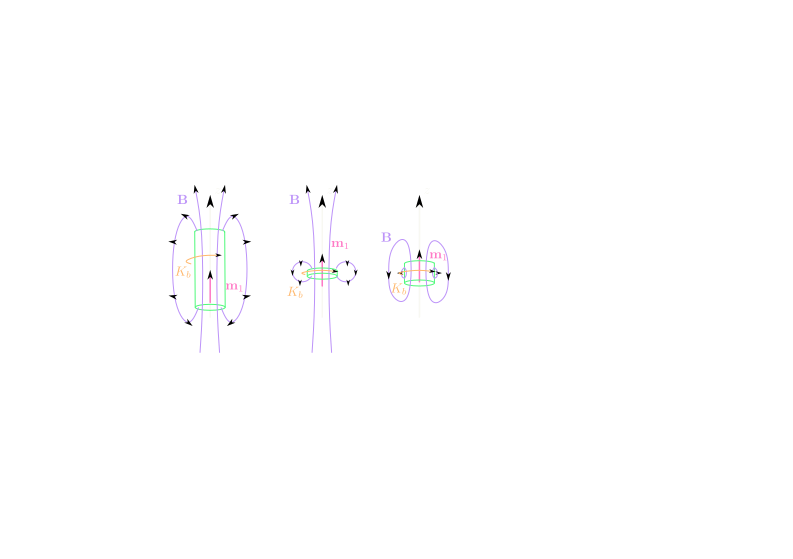
\includegraphics[width=0.8\textwidth]{hw10_2.pdf}
    \caption{(left) $L \gg a$, (center) $L \ll a$, and (right) $L = a$}
    \label{fig:hw10_2}
\end{figure*}
This is the same as the bar electret but with opposite directions for the ($\vb B$ vs. $\vb D$) field produced

\newpage
\begin{figure*}[ht]
    \centering
    \begin{subfigure}{0.45\textwidth}
        \centering
        \includegraphics[width=\textwidth]{hw10_3.png}
    \end{subfigure}
    \hfill
    \begin{subfigure}{0.45\textwidth}
        \centering
        \includegraphics[width=0.7\textwidth]{hw10_4.png}
    \end{subfigure}
    \caption{Superposition of torus and square loop with reversed current}
    \label{fig:hw10_3}
\end{figure*}
\paragraph{6.10} For an iron rod of length $L$ and square cross section of side length $a$ with Magnetization $\vb M$ and bent around
in a circle with gap $w$: Assuming $w \ll a \ll L$ find the magnetic field at the center of the gap:
The magnetization of the torus is $\vb M = M \vu*\phi$ so the magnetic field
of the torus is
\begin{align*}
    \vb B = \mu_0 \vb M
\end{align*}
% hw10_4.png
The magnetic field at the center of the square loop is equivalent to four times the magnetic field of a straight wire (From Griffiths Example 5.5):
\begin{align*}
    B = -4 \frac{\mu_0 I}{4\pi R} \sin\theta \eval_{\theta = -\pi/4}^{\pi/4} = \frac{\mu_0 I}{\pi R} \qt(\sqrt{2}/2 + \sqrt{2}/2) = \frac{\sqrt{2}\mu_0 I}{\pi R}
\end{align*}
where the square loop has a current $I = m / a$ where $M \equiv m / V$
\begin{align*}
    \implies I = \frac{MV}{a} = M w
\end{align*}
and $R = a / 2$ so
\begin{align*}
    B = -\frac{\sqrt{2}\mu_0 M w}{\pi a / 2} = -\frac{2\sqrt{2}\mu_0 M w}{\pi a}
\end{align*}
The magnetic field is a superposition of the torus and square loop with reversed current
\begin{align*}
    \boxed{
        \vb B = \mu_0 \vb M - \frac{2\sqrt{2}\mu_0 \vb M w}{\pi a}
    }
\end{align*}

\newpage
\paragraph{6.25} For two charged $q$ magnetic dipoles $\vb m$ constrained to move on the
$z$ axis, they electrically repel and magnetically attract:
\begin{itemize}
    \item [(a)] The equilibrium separation distance: From Coloumbs law the electric force is
    \begin{align*}
        \vb F_e = \ke \frac{q^2}{z^2} \vu z
    \end{align*}
    and the magnetic force is (From Prob. 6.3)
    \begin{align*}
        \vb F_m = \grad(\vb m \vdot \vb B) = - \frac{3\mu_0}{2\pi} \frac{m^2}{z^4} \vu z
    \end{align*}
    so at equilibrium
    \begin{align*}
        \vb F_e = -\vb F_m \implies \ke \frac{q^2}{z^2} = \frac{3\mu_0}{2\pi} \frac{m^2}{z^4} \implies z = \frac{m\sqrt{6\epsilon_0 \mu_0}}{q}
    \end{align*}
    where we can use the fact that $\epsilon_0 \mu_0 = 1 / c^2$ to rewrite the equilibrium separation distance as
    \begin{align*}
        \boxed{z = \sqrt{6} \frac{m}{qc}}
    \end{align*}
    \item [(b)] For two electrons, we can use the magnetic moment of an electron, i.e, the ``Bohr magneton'' \href{https://en.wikipedia.org/wiki/Bohr_magneton}{Wiki},
    \begin{align*}
        m = \frac{e \hbar}{2m_e}
    \end{align*}
    withe with electron charge $q = e = \qty{1.6e-19}{C}$, mass $m_e = \qty{9.11e-31}{kg}$, reduced planck constant $\hbar = \qty{1.05e-34}{J s}$, and speed of light $c = \qty{3e8}{m/s}$:
    \begin{align*}
        z &= \sqrt{6} \frac{e\hbar}{2m_e q c} \\
        &= \sqrt{6} \frac{\hbar}{2m_e c} \\
        &= \sqrt{6} \frac{\qty{1.05e-34}{J s}}{2 \qty{9.11e-31}{kg} \qty{3e8}{m/s}} \\
        &= \qty{4.72e-13}{m}
    \end{align*}
    \item [(c)] Since the equilibrium separation distance is much smaller than the Bohr radius $a_0 = \qty{5.29e-11}{m}$,
    there is \emph{no stable bound state of two electrons}
\end{itemize}
\end{document}